\section{Связность в орграфе: различные виды связности, примеры. Компоненты сильной связности. 
Алгоритм Косарайю нахождения компонент сильной связности. Граф конденсации Применить 
алгоритм к орграфу, найти граф конденсации.}

\begin{definition}
    Ориентированный граф называется \textit{сильно связным}, если для
    любых двух вершин $v$, $u$ графа есть маршрут из $v$ в $u$ и наоборот.
\end{definition}

\begin{definition}
    Ориентированный граф $G$ называется \textit{односторонне связным},
    если для любых двух вершин $v$, $u$ существует хотя бы один из маршрутов из
    одной вершины в другую.
\end{definition}

\begin{definition}
    Ориентированный граф называется \textit{слабо связным}, если
    соответствующий ему неориентированный граф, в котором нет ориентации
    рёбер, является связным.
\end{definition}

Если задать каждому из этих трех определений бинарное отношение, то
только один из заданных отношений на множестве вершин ориентированного
графа является отношением эквивалентности.

\begin{theorem}
    Отношение сильной связности на множестве вершин ориентированного
    графа является отношением эквивалентности.
\end{theorem}

Поэтому все вершины распадаются на компоненты сильной связности --
такие подмножества, что внутри одной компоненты все вершины сильно
связаны, а между вершинами разных компонент сильной связности нет.

Пример графа с тремя компонентами сильной связности.
\begin{figure}[h]
    \centering
    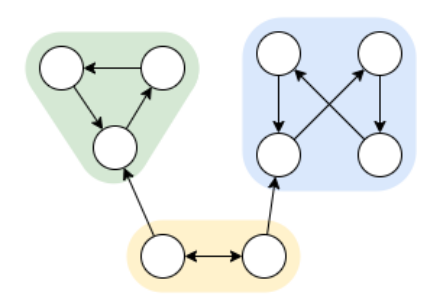
\includegraphics[scale=0.35]{16.png}
\end{figure}

Самый простой пример сильно-связной компоненты -- это цикл. Но это может
быть и полный граф, или сложное пересечение нескольких циклов.

\begin{definition}
    \textit{Транспонирование (инвертирование) графа} -- смена
    направлений всех ребер в графе на противоположные.
\end{definition}

Заметим, что инвертирование в графе не меняет компонент сильной связности
графа.

\textbf{Алгоритм Косарайю для нахождения компонент сильной связности}
\begin{enumerate}[left=0.0em, labelsep=1em, topsep=0.0em, itemsep=0pt, parsep=0.5em]
    \item Запускаем алгоритм DFS (обхода графа в глубину). Фиксируем время
    для вершины, когда она становилась черной(тупиковой). Обозначаем это
    время $T_{out}$ Получаем последовательность вершин в том порядке, в котором они
    становились черными.
    \item Записываем последовательность вершин, в порядке убывания времени
    $T_{out}$.
    \item Инвертируем граф.
    \item Запускаем DFS к инвертированному графу для последовательности
    вершин в порядке, полученном в шаге 2. Всем достижимым из текущей
    вершины вершинам присваиваем ее номер (это будут компоненты сильной
    связности)
\end{enumerate}

Пример алгоритма:
\begin{figure}[h]
    \centering
    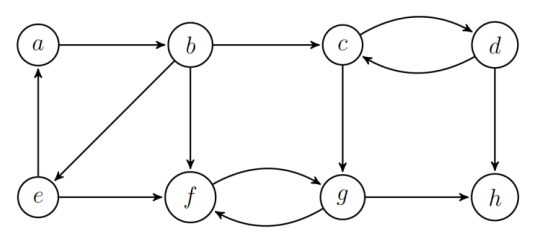
\includegraphics[scale=0.35]{16_2.png}
\end{figure}

Имеем следующие компоненты сильной связности: \\
$\set{a,e,b},\set{f,g},\set{c,d},\set{h}$

\newpage
Часто рассматривают граф, составленный из самих компонент сильной
связности, а не индивидуальных вершин. Очевидно, такой граф уже будет
ациклическим, и с ним проще работать. Задачу о сжатии каждой компоненты
сильной связности в одну вершину называют \textit{конденсацией графа}.

\textit{Графом конденсации или графом Герца или конденсацией ориентированного
графа} $G$ называют такой ориентированный граф ${G}'$ вершинами которого
служат компоненты сильной связности $G$, а дуга в ${G}'$ между двумя вершинами
проводится только если в графе $G$ существует хотя бы одна дуга между
вершинами, входящими в соответствующие компоненты связности.

Для графа предыдущего примера графом конденсации является следующий граф:
\begin{figure}[h]
    \centering
    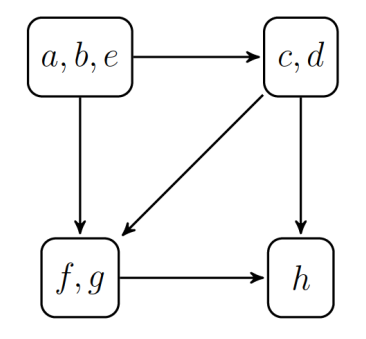
\includegraphics[scale=0.35]{16_3.png}
\end{figure}